\chapter{Markov Model: Analytical Validation of Game Dynamics}
Building upon the empirical insights into Snakes and Ladders game dynamics from agent-based simulations in Chapter 3, this chapter introduces a complementary analytical approach: a Markov Chain model. This chapter details the development, validation, and application of this model to rigorously predict expected game length, win probabilities, and steady-state distributions. Crucially, this Markovian framework serves to analytically verify the empirical findings from our simulations, thereby establishing a more robust and multifaceted understanding of the game's underlying mechanics.

\section{What are Markov Chains}
At its core, a Markov chain is a mathematical construct describing a system transitioning between discrete states in a sequential, chain-like manner. The defining characteristic, and analytical power, of a Markov chain lies in its ‘memoryless’ property: future state transitions depend solely on the current state, irrespective of the sequence of states that preceded it. In the context of Snakes and Ladders, we conceptualise each tile on the board as a distinct state. The probabilistic transition from one tile to the next is governed by the outcome of a dice roll, rendering the game dynamics amenable to Markovian analysis.

By adopting this framework, we can mathematically represent the inherent randomness of dice rolls and the deterministic rules of snake and ladder placements. This allows us to move beyond empirical observation and derive analytical expressions for key performance indicators, offering a powerful means of validating and extending our simulation-based research.

\section{Fundamental Concepts}
To ensure clarity and precision in our model description, it is essential to define the core concepts underpinning our Markovian approach:
\begin{enumerate}
	\item \textbf{States:} Each tile on the Snakes and Ladders board, indexed from 0 to $N$ (where $N$ is the board size), is defined as a unique state within our Markov model. State 0 represents the starting position, and state $N$ corresponds to the final tile, the absorbing goal state.
	\item \textbf{Transitions:} Game progression is modelled as probabilistic transitions between these states. Transitions occur in discrete steps, driven by dice rolls. Each roll of a fair six-sided die produces an outcome $k \in \{1, 2, 3, 4, 5, 6\}$, each with an equal probability of $\frac{1}{6}$. Adding this outcome to the current tile number determines a tentative next position, subject to board boundaries and entity adjustments.
	\item \textbf{Absorbing State:} The final tile, state $N$, is designated as an absorbing state. Once a player reaches or surpasses tile $N$, the game concludes, and the player remains in this state indefinitely. This is mathematically represented by a self-loop in the transition matrix, with a probability of 1.
	\item \textbf{Memorylessness (Markov Property):} The defining ‘memoryless’ property dictates that the probability of transitioning to any future state depends exclusively on the current state. The history of previous moves or states is irrelevant. This assumption is valid for Snakes and Ladders, as each dice roll and subsequent move are probabilistically independent of prior game events. This Markovian property significantly simplifies the mathematical analysis, allowing us to construct a tractable and predictive model.
\end{enumerate}

\section{Constructing the Transition Matrix}
The core of our Markov model is the transition matrix, $P$, a square matrix of size $(N-(N_s + N_l)) \times (N-(N_s + N_l))$, where $N$ is the board size. Each entry $P(i,j)$ quantifies the probability of transitioning from state $i$ to state $j$ in a single turn. To maintain the state space and focus on board position transitions, we do not treat snake heads or ladder bases as distinct states. For baseline analysis within this chapter, we configure the board with 10 snakes ($N_S$) and 10 ladders ($N_L$), with their lengths assigned randomly using the fixed start and end points methodology detailed in Chapter 2.

\subsection{Methodology}
For each non-absorbing state $i < N$:
\begin{enumerate}
	\item \textbf{Dice Roll Simulation:} We simulate the roll of a fair six-sided die, generating an outcome $k \in \{1, 2, 3, 4, 5, 6\}$, each with a probability of $\frac{1}{6}$.
	\item \textbf{Tentative Movement:} A tentative next state is calculated by adding the dice roll outcome $k$ to the current state $i$. Boundary conditions are applied: if the tentative state exceeds the board size $N$, the excess is reflected back onto the board, ensuring the player remains within valid tile positions.
	\item \textbf{Entity-Based Adjustment:} We then check if the tentative next state coincides with the start of a snake or the base of a ladder, based on the pre-defined board layout. If so, the state is immediately updated to the corresponding snake tail or ladder top, respectively.
	\item \textbf{Probability Assignment:} For each dice outcome $k$, the transition probability ($\frac{1}{6}$) is added to the matrix entry $P(i, j)$, where $j$ represents the final state reached after all movement and entity-based adjustments.
\end{enumerate}

For the absorbing state $N$, the transition matrix row is configured to represent absorption: $P(N, N) = 1$, and $P(N, j) = 0$ for all $j \neq N$. This ensures that once the final state is reached, the probability of transitioning to any other state is zero.

Mathematically, for non-absorbing states $i < N$, the transition probability is expressed as:
\[
P(i, j) = \sum_{k=1}^{6} \frac{1}{6} \cdot \mathbf{1}\{f(i,k) = j \}
\]
where $f(i,k)$ is a function encapsulating the game's movement rules: it computes the next state $j$ reached from state $i$ after rolling $k$, incorporating boundary reflections and snake/ladder adjustments. The indicator function $\mathbf{1}\{\cdot\}$ evaluates to 1 if the condition is true, and 0 otherwise.

For the absorbing state $N$, the transition probabilities are deterministic:
\[
P(N, N) = 1, \quad P(N, j) = 0 \quad \forall j \neq N.
\]
This formulation guarantees that each row of the transition matrix sums to unity, a fundamental property of stochastic matrices and Markov chains.

\section{Analytical Derivation of Game Metrics}

With the transition matrix constructed, we can analytically derive key game metrics using matrix-based methods. Specifically, we leverage the concept of the fundamental matrix to calculate expected game turns and estimate win probabilities.

\subsection{Fundamental Matrix and Expected Turns}

To calculate the expected number of turns to reach the absorbing state, we first partition the transition matrix $P$ into submatrices corresponding to transient (non-absorbing) and absorbing states. Let $Q$ be the submatrix representing transitions between transient states, and $R$ be the submatrix for transitions from transient to absorbing states. The fundamental matrix $N$, central to our analysis, is then computed as:
\[
N = (I - Q)^{-1}
\]
where $I$ is the identity matrix of the same dimension as $Q$. The entry $N(i, j)$ of the fundamental matrix provides the expected number of times the system visits transient state $j$ before absorption, starting from transient state $i$.

The expected number of turns, $t$, to reach the absorbing state from a starting state $i$ is derived by summing the entries in the $i^{th}$ row of the fundamental matrix $N$ and multiplying by a column vector of ones, $\mathbf{1}$:
\[
t_i = (N \cdot \mathbf{1})_i = \sum_{j} N(i, j)
\]
For a standard Snakes and Ladders game starting at state 0, the expected number of turns to reach the final tile is:
\[
t = t_0 = \sum_{j} N(0, j)
\]
This sum represents the total expected number of steps spent in transient states before absorption, effectively quantifying the average game duration in turns.

\subsection{Win Probabilities within Turn Limits}

Beyond expected game duration, we extend the Markov model to estimate win probabilities within specified turn limits, providing a more nuanced measure of game hardness. Agent-based simulations empirically estimate win probabilities for turn limits of $N/2$, $N/3$, and $N/4$ (where $N$ is board size) by tracking game completion rates within these thresholds over numerous trials. The Markov model, through iterative state transitions, provides a computationally derived estimate of these win probabilities. While a direct analytical derivation of win probability distributions from the fundamental matrix is mathematically complex, our iterative approach offers robust estimates, allowing for a direct comparison with simulation results and further validation of the model's predictive power.

\section{Validation: Markov Model vs. Agent-Based Simulations}
To rigorously validate our Markov Chain model, we compared its analytical predictions against empirical results from the agent-based simulations detailed in Chapter 3. This section presents a comparative analysis of expected game turns, win probabilities, and game turn distributions.

\subsection{Comparative Analysis of Expected Turns}

A key validation point is the comparison of analytically calculated expected game turns with the average game turns observed in agent-based simulations. For a representative board configuration (Figure \ref{fig:boardlayout}), simulations across 10,000 games yielded an average game duration of \textbf{33.99 turns}. Strikingly, the expected number of turns derived from our Markov model's fundamental matrix is \textbf{33.72 turns}. This remarkable concordance, with a negligible percentage difference, provides strong empirical validation for the Markov chain model's accuracy in predicting average game length in Snakes and Ladders. This analytical verification enhances the credibility of the simulation-based findings presented in Chapter 3, demonstrating convergent validity across methodological approaches.

\begin{figure}
	\centering
	\includegraphics[width=0.7\linewidth]{"../Markov Modelling/Data/BoardLayout"}
	\caption{Representative Board Layout for Model Validation: Snakes and Ladders configuration used for comparing Markov model predictions with agent-based simulation results.}
	\label{fig:boardlayout}
\end{figure}

\subsection{Comparative Analysis of Win Probabilities}

Further validation is achieved by comparing win probabilities within specified turn limits, calculated using both agent-based simulations and the Markov model. Figure \ref{fig:winprobability_NsFixed_05} presents a comparison of win probabilities for varying board sizes at a fixed Ns/Nl ratio of 0.5 (Ns fixed).  The plot juxtaposes win probabilities derived from agent-based simulations against those predicted by the Markov model for turn limits of N/2, N/3, and N/4.

\begin{figure}[th]
	\centering
	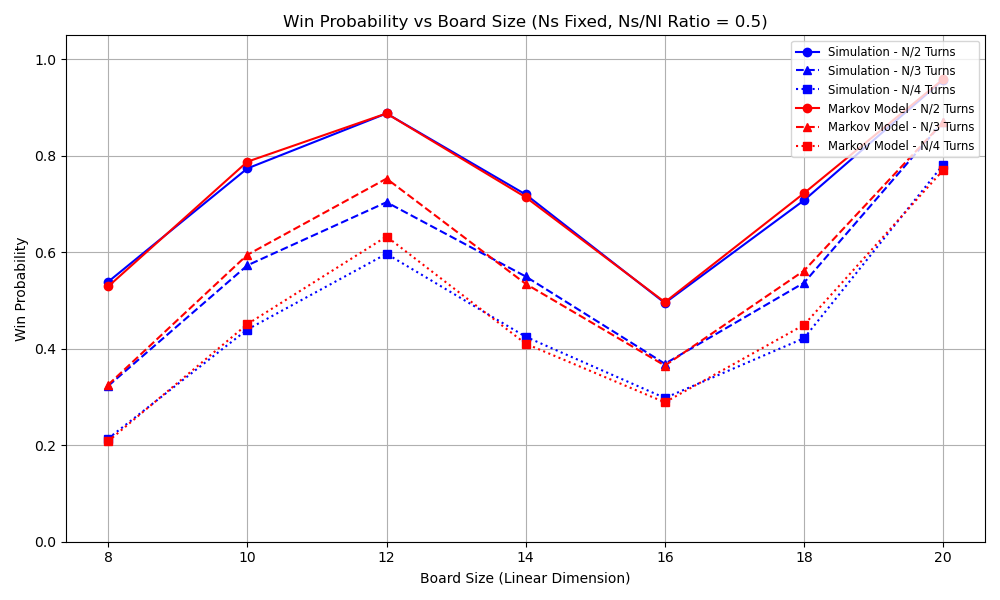
\includegraphics[width=0.8\textwidth]{"../Markov Modelling/Code/plots/plots/chapter4_validation/win_probability_plot_NsFixed_05.png"}
	\caption{\textbf{Win Probability vs Board Size} Comparison of win probabilities within N/2, N/3, and N/4 turns, derived from agent-based simulations and Markov model predictions, demonstrating a high degree of agreement.}
	\label{fig:winprobability_NsFixed_05}
\end{figure}

As illustrated in Figure \ref{fig:winprobability_NsFixed_05}, the Markov model's predictions for win probabilities closely align with the empirical results from agent-based simulations. Both methodologies demonstrate a similar trend: win probabilities within limited turns generally \textit{increase} as board size expands, despite the longer average game times associated with larger boards, as discussed in Chapter 3.  This counter-intuitive finding, validated by both simulation and analytical methods, underscores the nuanced impact of board size on game dynamics. The close quantitative agreement between the predicted and simulated win probabilities further bolsters confidence in the Markov model's ability to capture essential aspects of game hardness beyond just average game duration.  Further comparisons across other Ns/Nl ratios and density configurations would similarly strengthen this validation.

\subsection{Comparative Distribution Analysis: Game Turns}

A more granular validation of the Markov model is achieved by comparing the full distribution of game turns. Figure \ref{fig:frequencydistributionMarkov} presents a comparative view of game turn distributions, juxtaposing empirical distributions from 10,000 agent-based simulations against the distribution derived from the Markov model. The Markov-derived distribution is generated by probabilistically simulating game progression through the transition matrix for 10,000 iterations, mirroring the simulation approach.

\begin{figure}[th]
	\centering
	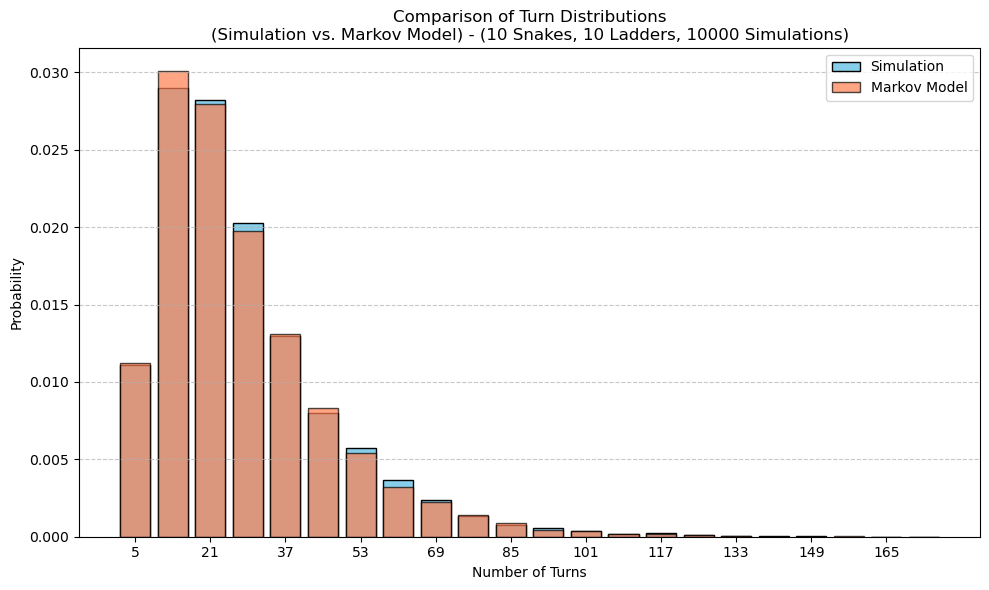
\includegraphics[width=0.7\textwidth]{"../Markov Modelling/Data/FrequencyOveralyed.png"}
	\caption{\textbf{Distribution of Game Turns: Simulation vs. Markov Model (10 Snakes, 10 Ladders, 10,000 Games):} Probability distributions of game turns from agent-based simulations and Markov model-based predictions exhibit a high degree of congruence, demonstrating model validity.}
	\label{fig:frequencydistributionMarkov}
\end{figure}

Visual inspection of Figure \ref{fig:frequencydistributionMarkov} reveals a strong qualitative agreement between the two distributions. Both exhibit a characteristic right-skewed pattern, peaking in the 10-20 turn range and displaying a long tail extending towards higher turn counts. This close mirroring of distributional shapes and central tendencies provides compelling evidence that the Markov model accurately captures the stochasticity and overall dynamics of game progression in Snakes and Ladders. The histogram derived from agent-based simulations closely aligns with the distribution predicted by the Markov model, further solidifying the model's capacity to represent the game's probabilistic nature.

\subsection{Steady-State Distribution and Gameplay Hotspots}

The steady-state distribution, derived analytically from the Markov model, offers insights into the long-term probabilities of tile occupation, representing the equilibrium state of the game over infinite plays. Figure \ref{fig:steady_state_heatmap_chapter3} (b) visualises this steady-state distribution as a heatmap, juxtaposed with the Tile Visit Frequency Heatmap (Figure \ref{fig:steady_state_heatmap_chapter3} (a)) empirically derived from agent-based simulations.

\begin{figure}[ht]
	\centering
	\subfloat[]{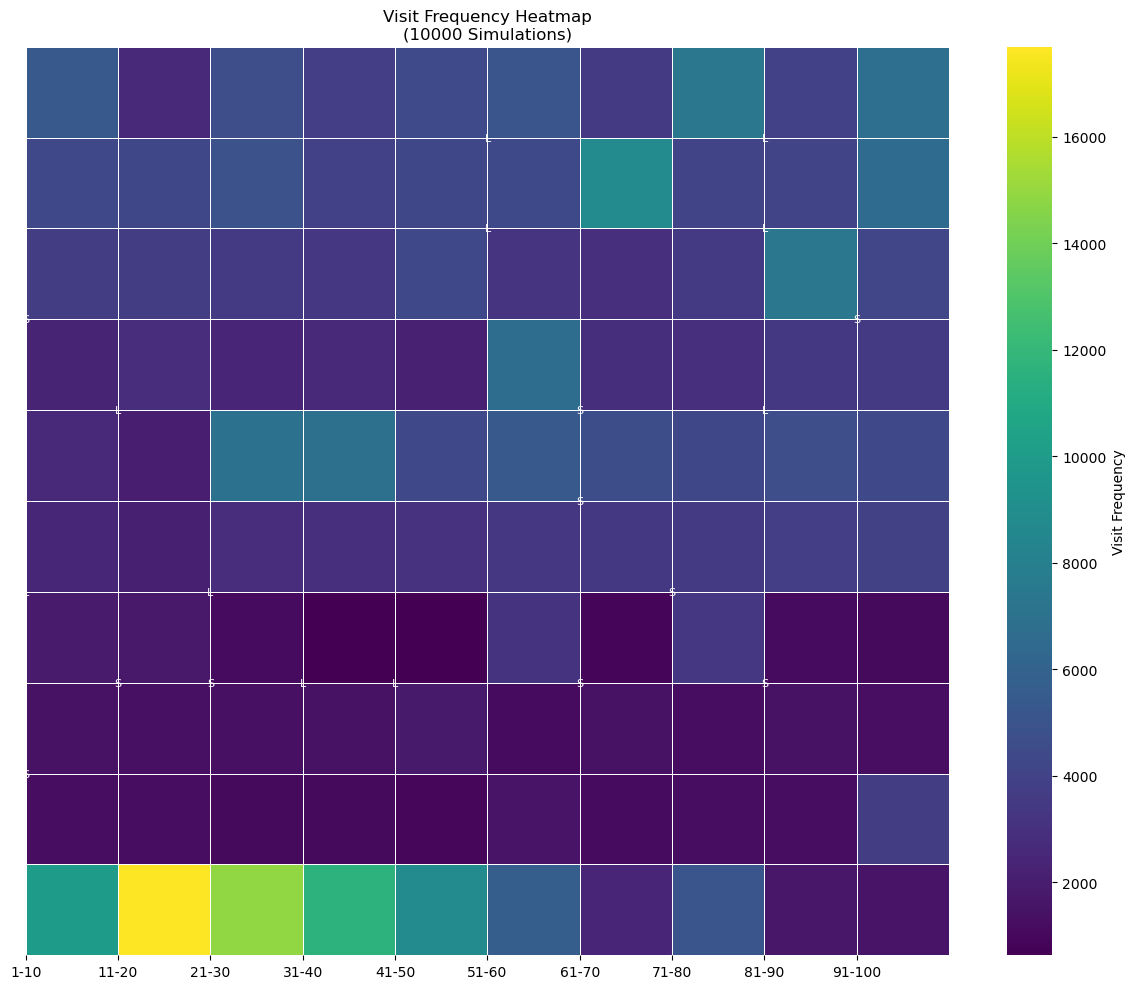
\includegraphics[width=0.45\textwidth]{"../Markov Modelling/Data/TileVisitHeatmap.png"}}
	\subfloat[]{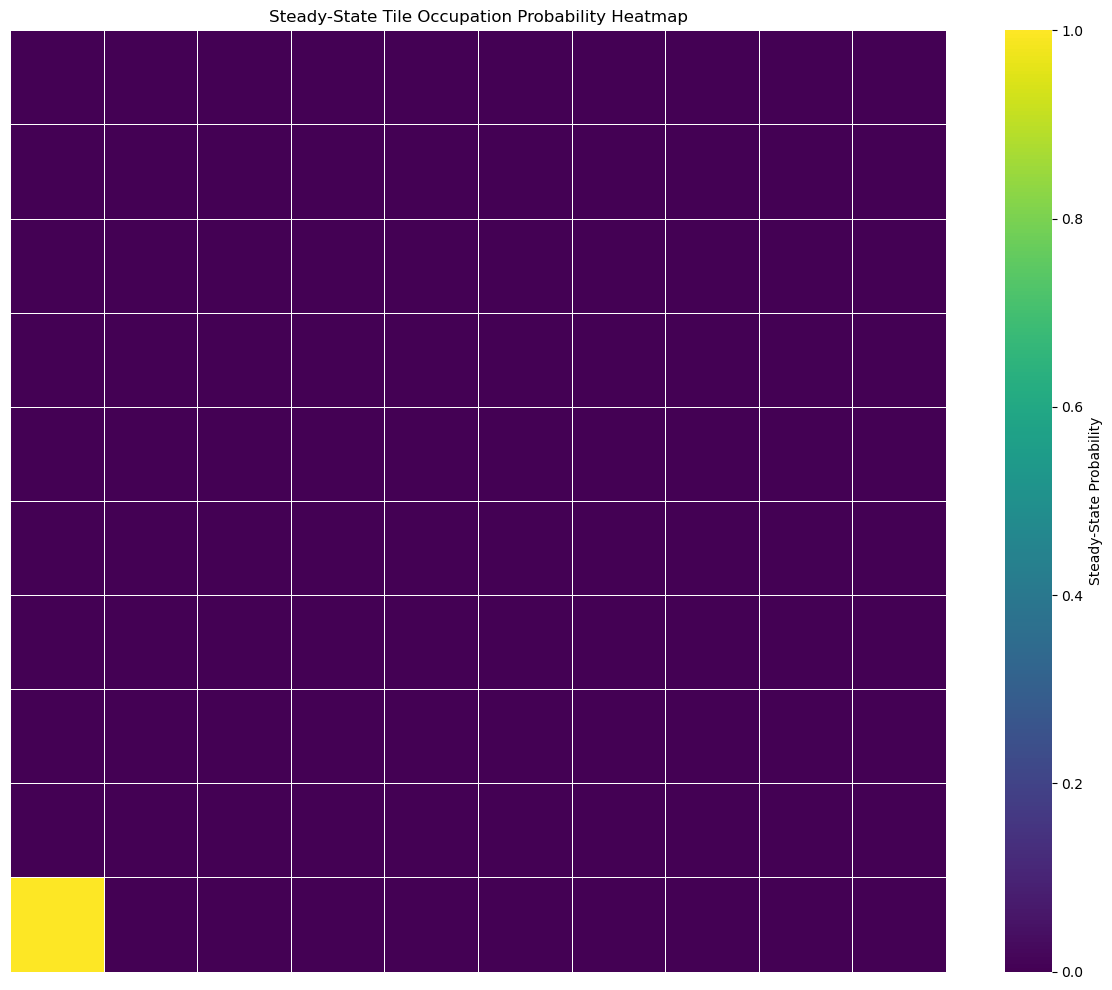
\includegraphics[width=0.45\textwidth]{"../Markov Modelling/Data/SteadyStateHeatmap.png"}}
	\caption{Heatmap Comparison: (a) Tile Visit Frequency Heatmap from Agent-Based Simulations, empirically highlighting gameplay hotspots; (b) Steady-State Tile Occupation Probability Heatmap from Markov Model, illustrating long-term equilibrium.}
	\label{fig:steady_state_heatmap_chapter3}
\end{figure}

As theoretically expected for a well-formulated absorbing Markov chain, the Steady-State Heatmap (Figure \ref{fig:steady_state_heatmap_chapter3} (b)) demonstrates a probability of 1.0 concentrated on tile 100 (bottom-right corner), with probabilities for all other tiles approaching zero. This analytically confirms that, in the long run, the game predictably terminates at the absorbing winning state.

In contrast, the Tile Visit Frequency Heatmap from simulations (Figure \ref{fig:steady_state_heatmap_chapter3} (a)) empirically reveals tiles frequently visited during active gameplay. This heatmap highlights gameplay hotspots and tiles of relative importance during a typical game session. While the Steady-State Heatmap represents the game's theoretical long-term behaviour, the Tile Visit Frequency Heatmap offers more practical insights into tile occupation patterns and player experience during actual gameplay. Together, they provide complementary perspectives on game dynamics and tile importance.

\subsection{Analytical Efficiency in Game Time Derivation}

A significant advantage of the Markov model is its analytical efficiency in deriving expected game time. Unlike agent-based simulations, which require computationally intensive repeated trials to approximate average game durations, the Markov model offers a direct, deterministic calculation through fundamental matrix analysis. This analytical solution provides a rigorous and computationally efficient alternative for determining average game durations across diverse board configurations and parameter settings. The demonstrated close agreement between the analytical expected turns and simulation-based average turns validates the Markovian approach as not only accurate but also a computationally advantageous tool for analysing game time in Snakes and Ladders.

\section{Conclusion: Validation and Utility of the Markov Model}

This chapter has successfully developed and rigorously validated a Markov Chain model for Snakes and Ladders. Through comparative analysis, encompassing expected game turns, win probabilities, game turn distributions, and steady-state behaviour, we have demonstrated a strong convergence between the analytical predictions of the Markov model and the empirical findings from agent-based simulations. This robust validation reinforces the accuracy and reliability of both methodological approaches.

The Markov model provides a powerful analytical framework for understanding and quantifying Snakes and Ladders game dynamics. Its capacity to derive expected game time and steady-state distributions analytically, coupled with its validation against empirical simulations for win probabilities and turn distributions, establishes its utility as a valuable tool for game analysis and design. Moreover, the model's computational efficiency offers a significant advantage for rapid evaluation of diverse game configurations and parameter variations, paving the way for more normative investigations into optimal board design and game balancing, which we will address in subsequent chapters. The validated Markovian approach, therefore, not only enhances our understanding of Snakes and Ladders but also provides a robust analytical foundation for further prescriptive research in game design and mechanics.